\documentclass[a4paper,10pt]{article}
\usepackage[utf8]{inputenc}
\usepackage[spanish]{babel}
\usepackage[affil-it]{authblk}
\usepackage{enumerate}
\usepackage{graphicx}
\usepackage{hyperref}
\usepackage{amsmath}
\usepackage{amssymb}
\usepackage{cancel}
\usepackage[usenames, dvipsnames]{color}
\usepackage{tikz}
\usepackage{multimedia}
\usepackage{subcaption} %Multiple images
\usepackage{multicol} % Multiple columns
\usepackage{float}
\usepackage{cleveref}
\usepackage[margin=1.4in]{geometry}
\usepackage[labelfont=bf]{caption}
\usetikzlibrary{calc}
\numberwithin{equation}{section}

%Columns separation
\setlength{\columnsep}{1cm}

%Indentation
\setlength{\parindent}{0ex}

%Multiple References

\usepackage{xparse}
\ExplSyntaxOn
\NewDocumentCommand{\mref}{m}{\quinn_mref:n {#1}}
\seq_new:N \l_quinn_mref_seq
\cs_new:Npn \quinn_mref:n #1
 {
  \seq_set_split:Nnn \l_quinn_mref_seq { , } { #1 }
  \seq_pop_right:NN \l_quinn_mref_seq \l_tmpa_tl
  ( % print the left parenthesis
  \seq_map_inline:Nn \l_quinn_mref_seq
    { \ref{##1},\nobreakspace } % print the first references
  \exp_args:NV \ref \l_tmpa_tl 
  ) 
 }
\ExplSyntaxOff


%Boxes

\newcommand*{\boxcolor}{blue}
\makeatletter
\renewcommand{\boxed}[1]{\textcolor{\boxcolor}{%
\tikz[baseline={([yshift=-1ex]current bounding box.center)}] \node [rectangle, minimum width=1ex,rounded corners,draw] {\normalcolor\m@th$\displaystyle#1$};}}
 \makeatother

%Constantes
\newcommand{\euler}{\mathrm{e}}
\newcommand{\im}{i}

%Lemas, teoremas, definiciones y pruebas
\newcommand{\definicion}{\textbf{Definición: }}
\newcommand{\lema}{\textbf{Lema: }}
\newcommand{\teorema}{\textbf{Teorema: }}
\newcommand{\prueba}{\textbf{Prueba: }}


%opening
\title{Mecánica Clásica Tarea \# 6}
\author{Favio Vázquez\thanks{Correo: favio.vazquezp@gmail.com}}\affil{Instituto de Ciencias Nucleares. Universidad Nacional Autónoma de México.}
\date{}

\begin{document}

\makeatletter
\def\@maketitle{%
  \newpage
  \null
  \vskip 2em%
  \begin{center}%
  \let \footnote \thanks
    {\Large\bfseries \@title \par}%
    \vskip 1.5em%
    {\normalsize
      \lineskip .5em%
      \begin{tabular}[t]{c}%
        \@author
      \end{tabular}\par}%
    \vskip 1em%
    {\normalsize \@date}%
  \end{center}%
  \par
  \vskip 1.5em}
\makeatother

\maketitle

\section{Problema 1}

Una partícula de masa $m$ se mueve constreñida a la superficie de un paraboloide de 
revolución que tiene su abertura hacia arriba en presencia del campo de la gravedad. 
Calcule las fuerzas de constricción.

\vspace{.3cm}

\underline{Solución:} \vspace{.3cm}

Para visualizar mejor el problema al cual nos enfrentamos, se muestra en la figura 
de abajo una partícula de masa $m$ constreñida a moverse en dicho paraboloide.

\begin{figure}[H]
 \center 
 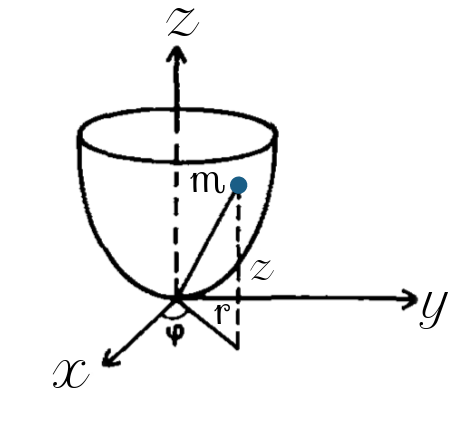
\includegraphics[scale=0.5]{problema1fig1}
 \caption{Partícula de masa $m$ se mueve constreñida a la superficie de un paraboloide de 
revolución}
\label{fig:problema1fig1}
\end{figure}

Debido a las simetrías involucradas en este problema, utilizaremos coordenadas cilíndricas 
polares para resolverlo. Tenemos entonces las siguientes transformaciones de coordenadas,

\begin{align}
 x &= r\cos{\phi}, \\
 y &= r\sen{\phi}, \\
 z &= z.
 \label{eq:transfCoordenadasParab}
\end{align}

Por otra parte, tenemos la constricción holonómica de que la partícula debe moverse 
en la superficie del paraboloide de revolución, que podemos expresar como

\begin{equation}
 x^2 + y^2 = \alpha z.
\end{equation}

Pero en las coordenadas que estamos utilizando

\begin{equation}
 x^2 + y^2 = r^2,
\end{equation}

entonces la constricción se convierte en,

\begin{equation}
 z = \alpha r^2.
 \label{eq:constriccionParab}
\end{equation}

Siguiendo la receta lagrangiana calculemos ahora la energía cinética y la potencial 
en nuestras coordenadas generalizadas $(r,\phi,z)$. Recordemos que podemos escribir 
estas energías en coordenadas cartesianas como,

\begin{equation}
 T = \frac{1}{2}m(\dot{x}^2 + \dot{y}^2 +\dot{z}^2).
 \label{eq:energCinetParab1}
\end{equation}

\begin{equation}
 V = mgz.
 \label{eq:energPotenParab1}
\end{equation}

Debido a que la partícula se encuentra en un campo gravitacional uniforme. Expresemos 
ahora estas energías en términos de nuestras coordenadas generalizadas. Cabe resaltar 
que utilizaremos el método de los coeficientes indeterminados de Lagrange para obtener 
las fuerzas generalizadas, por lo cual haremos uso de la constricción en los momentos 
indicados por esta metodología. 

\vspace{.3cm}

Comencemos por obtener las derivadas temporales de \mref{eq:transfCoordenadasParab}, 
para introducirlas en \mref{eq:energCinetParab1},

\begin{align}
 \dot{x} = \dot{r}\cos{\phi} - r \dot{\phi}\sen{\phi}, \\
 \dot{y} = \dot{r}\sen{\phi} + r \dot{\phi}\cos{\phi}, \\
 \dot{z} = \dot{z}.
 \label{eq:derivTemprTransfCoordParab}
\end{align}

Introduciendo \mref{eq:derivTemprTransfCoordParab} en \mref{eq:energCinetParab1} obtenemos,

\begin{align}
 \begin{split}
  T &= \frac{1}{2}m [( \dot{r}\cos{\phi} - r \dot{\phi}\sen{\phi})^2
  + (\dot{r}\sen{\phi} + r \dot{\phi}\cos{\phi})^2 + \dot{z}^2], \\
  %  
  &= \frac{1}{2} m (\dot{r}^2\cos^2{\phi} - \cancel{2r\dot{r}\dot{\phi}\cos{\phi}\sen{\phi}} + 
  r^2\dot{\phi}^2 \sen^2{\phi} +  \dot{r}^2\sen^2{\phi} \\
  %
  &+ \cancel{2r\dot{r}\dot{\phi}\cos{\phi}\sen{\phi}}
  + r^2\dot{\phi}^2 \cos^2{\phi} + \dot{z}^2 ) \\
  %
  &= \frac{1}{2} m \left[ \dot{r}^2\cancelto{1}{(\sen^2{\phi} + \cos^2{\phi})}
  + r^2\dot{\phi}^2 \cancelto{1}{(\sen^2{\phi} + \cos^2{\phi})} + \dot{z}^2 \right]
  %%
 \end{split}
\end{align}

\begin{equation}
 \therefore T = \frac{1}{2}m(\dot{r}^2 + r^2\dot{\phi}^2 + \dot{z}^2)
 \label{eq:energCinetParab2}
\end{equation}










\section{Problema 2}

Considere la lagrangiana de una partícula de masa $m$ totalmente libre en el 
espacio tridimensional desde la perspectiva de un sistema inercial y desde la 
perspectiva de un sistema que está en rotación respecto al inercial, y en 
traslación respecto a la partícula (estos movimientos no son necesariamente uniformes). 
Establezca las ecuaciones de Lagrange en ambos sistemas y, a partir de estas ecuaciones, 
encuentre las expresiones para las fuerzas ficticias; identifique en particular 
las fuerzas: centrífuga, de Coriolis, y de Euler.

\vspace{.3cm}

\underline{Solución:} \vspace{.3cm}

\section{Problema 3}

Un girocompás es un instrumento que consisten de un cuerpo rígido simétrico, 
$(I_1 = I_2 \ne I_3)$ cuyo eje de simetría está constreñido a permanecer sobre 
un plano horizontal en la superficie de la Tierra, la que, naturalmente está en 
rotación en torno a su eje con un período de 24 horas. Suponga que un girocompás 
se encuentra en un punto de la Tierra de latitud $\phi$ y se pone, inicialmente, 
en rotación en torno a su eje de simetría con una velocidad angular $\omega_3$ cuando 
dicho eje apunta en una dirección arbitraria. Calcule una lagrangiana para este 
sistema. Demuestre que la velocidad de rotación en torno al eje de simetría, $\omega_3$,
permanece constante. Demuestre que si $\omega_3 > (I_1,I_3)\omega_0\cos{\phi}$ entonces 
el eje de simetría oscilará, de manera estable, en torno a la dirección norte-sur 
($\omega_0$ es la velocidad angular de la Tierra).

\vspace{.3cm}

\underline{Solución:} \vspace{.3cm}


\end{document}
